%!TEX root = main.tex
\chapter{Supplementary Results on Camera Calibration Estimation}     % numérotée
\label{annex5}

\DeclareGraphicsExtensions{.pdf,.jpeg,.png,.jpg}
\graphicspath{{annex5_figures/}}

%\hypertarget{a-perceptual-measure-for-deep-single-image-camera-calibration-2618-supplementary-material}{%
%\section{A Perceptual Measure for Deep Single Image Camera Calibration (\#2618) --- Supplementary Material}\label{a-perceptual-measure-for-deep-single-image-camera-calibration-2618-supplementary-material}}

The purpose of this annex is to extend the results presented in chapter~\ref{ch4}. Specifically, more results on horizon line estimation,
smoothed guided backpropagation and virtual object insertion are
provided.

\section*{Table of Contents}

\begin{enumerate}
\tightlist
\item
  \protect\hyperlink{he}{Horizon Line Estimations (extends fig.~\ref{fig:method_example_results})}
\item
  \protect\hyperlink{sgbp}{Smoothed Guided Backpropagation (extends fig.~\ref{fig:nn_analysis_smoothed-guided-back-propagation})}
\item
  \protect\hyperlink{study}{User Study Examples (extends fig.~\ref{fig:pstudy_overall_sensitivity})}
\item
  \protect\hyperlink{studyresults}{User Study Results (extends fig.~\ref{fig:pstudy_overall_sensitivity})}
\item
  \protect\hyperlink{voi}{Virtual Object Insertions (extends fig.~\ref{fig:applications_virtual_object_insertion})}
\item
  \protect\hyperlink{ablative}{Ablative study}
\end{enumerate}


\clearpage

\protect\hypertarget{he}{}{}

\hypertarget{horizon-line-estimations}{%
\section{Horizon Line Estimations}\label{horizon-line-estimations}}

In this section, we present additional horizon line estimations,
extending the results shown in fig.~\ref{fig:method_example_results}.

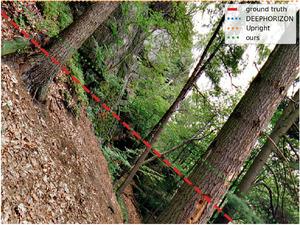
\includegraphics{horizon_estimation/thumb/pano_addiryhuippofz-1.jpg}
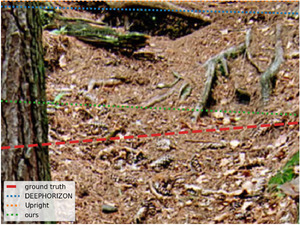
\includegraphics{horizon_estimation/thumb/pano_addiryhuippofz-4.jpg}
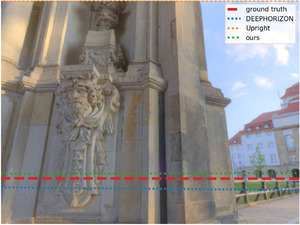
\includegraphics{horizon_estimation/thumb/pano_additeyvjdqubv-0.jpg}
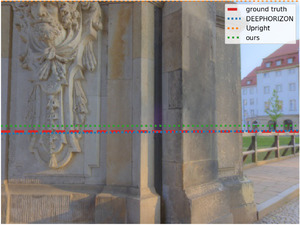
\includegraphics{horizon_estimation/thumb/pano_additeyvjdqubv-1.jpg}
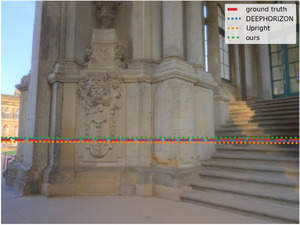
\includegraphics{horizon_estimation/thumb/pano_additeyvjdqubv-2.jpg}
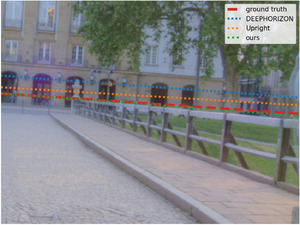
\includegraphics{horizon_estimation/thumb/pano_additeyvjdqubv-3.jpg}
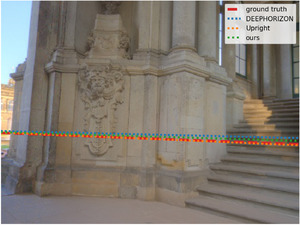
\includegraphics{horizon_estimation/thumb/pano_additeyvjdqubv-4.jpg}
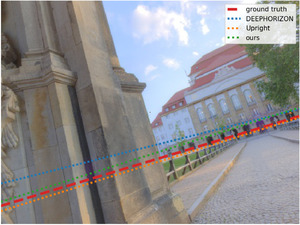
\includegraphics{horizon_estimation/thumb/pano_additeyvjdqubv-6.jpg}
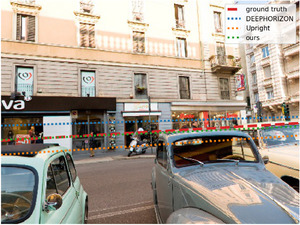
\includegraphics{horizon_estimation/thumb/pano_addiwhphxpexcd-0.jpg}
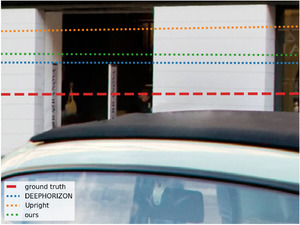
\includegraphics{horizon_estimation/thumb/pano_addiwhphxpexcd-1.jpg}
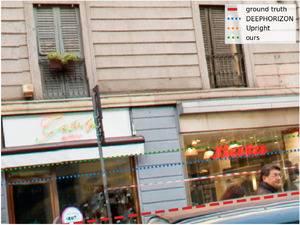
\includegraphics{horizon_estimation/thumb/pano_addiwhphxpexcd-2.jpg}
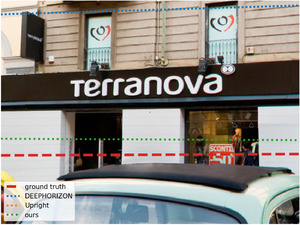
\includegraphics{horizon_estimation/thumb/pano_addiwhphxpexcd-3.jpg}
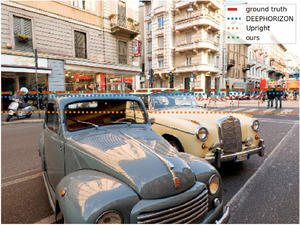
\includegraphics{horizon_estimation/thumb/pano_addiwhphxpexcd-5.jpg}
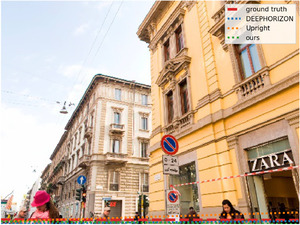
\includegraphics{horizon_estimation/thumb/pano_addiwhphxpexcd-6.jpg}
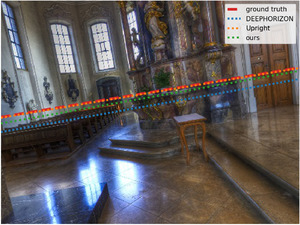
\includegraphics{horizon_estimation/thumb/pano_addiyhtujpaovr-0.jpg}
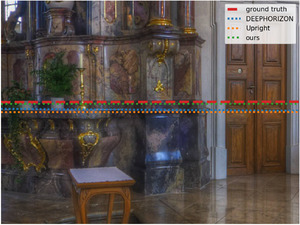
\includegraphics{horizon_estimation/thumb/pano_addiyhtujpaovr-3.jpg}
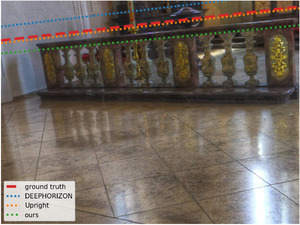
\includegraphics{horizon_estimation/thumb/pano_addiyhtujpaovr-4.jpg}
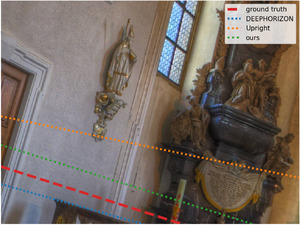
\includegraphics{horizon_estimation/thumb/pano_addiyhtujpaovr-5.jpg}
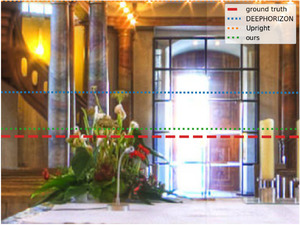
\includegraphics{horizon_estimation/thumb/pano_addiyhtujpaovr-6.jpg}
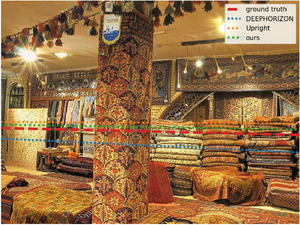
\includegraphics{horizon_estimation/thumb/pano_addjhelqxestdk-0.jpg}
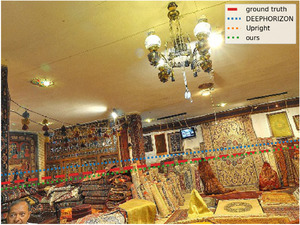
\includegraphics{horizon_estimation/thumb/pano_addjhelqxestdk-2.jpg}
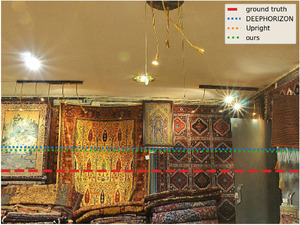
\includegraphics{horizon_estimation/thumb/pano_addjhelqxestdk-3.jpg}
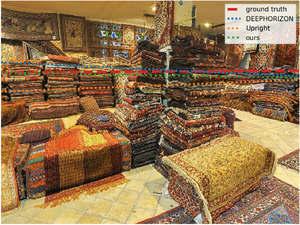
\includegraphics{horizon_estimation/thumb/pano_addjhelqxestdk-4.jpg}
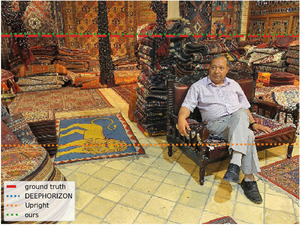
\includegraphics{horizon_estimation/thumb/pano_addjhelqxestdk-6.jpg}
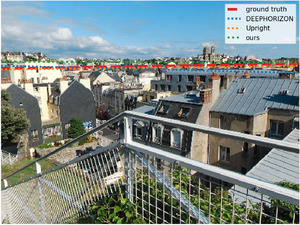
\includegraphics{horizon_estimation/thumb/pano_addkkzvqqxujqf-0.jpg}
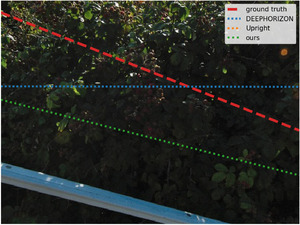
\includegraphics{horizon_estimation/thumb/pano_addkkzvqqxujqf-3.jpg}
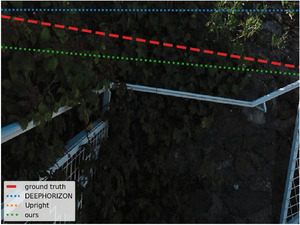
\includegraphics{horizon_estimation/thumb/pano_addkkzvqqxujqf-4.jpg}
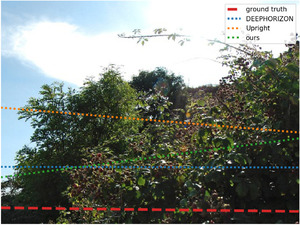
\includegraphics{horizon_estimation/thumb/pano_addkkzvqqxujqf-6.jpg}
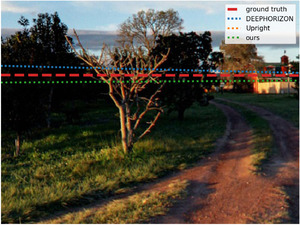
\includegraphics{horizon_estimation/thumb/pano_addknxbljsbxqc-0.jpg}
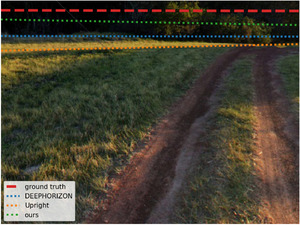
\includegraphics{horizon_estimation/thumb/pano_addknxbljsbxqc-1.jpg}


\clearpage

\protect\hypertarget{sgbp}{}{}

\hypertarget{smoothed-guided-backpropagation}{%
\section{Smoothed Guided Backpropagation}\label{smoothed-guided-backpropagation}}

In this section, we present additional smoothed guided backpropagation,
extending the results shown in fig.~\ref{fig:nn_analysis_smoothed-guided-back-propagation}.

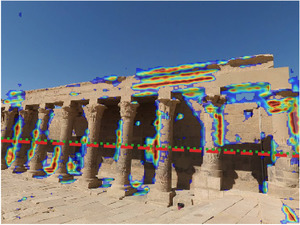
\includegraphics{sgbp/thumb/pano_addbhhhqoevobx-1.jpg}
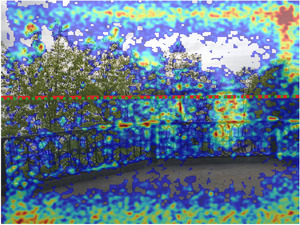
\includegraphics{sgbp/thumb/pano_addcepusvsloks-3.jpg}
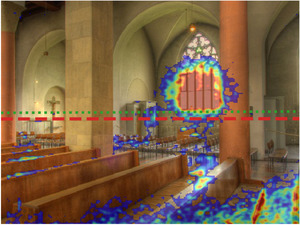
\includegraphics{sgbp/thumb/pano_addcvcjtwboiev-3.jpg}
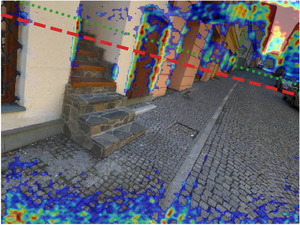
\includegraphics{sgbp/thumb/pano_addekhyhqjvbeb-0.jpg}
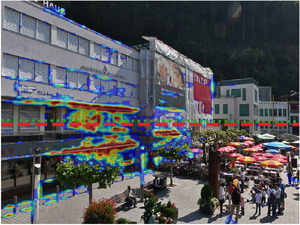
\includegraphics{sgbp/thumb/pano_addfjqyibbzulh-2.jpg}
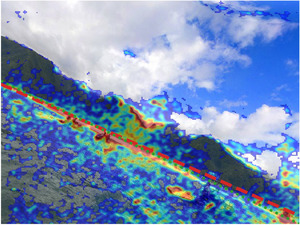
\includegraphics{sgbp/thumb/pano_addgasjevqjafh-1.jpg}
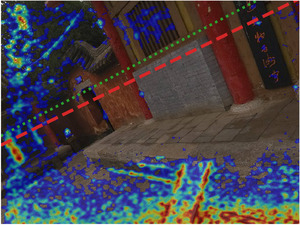
\includegraphics{sgbp/thumb/pano_addgtzfdddfgrh-2.jpg}
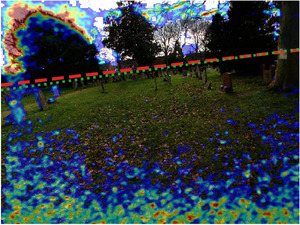
\includegraphics{sgbp/thumb/pano_addhxkomphqrlr-4.jpg}
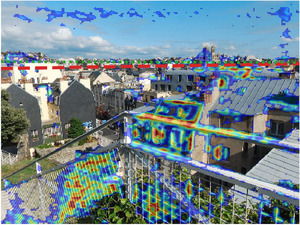
\includegraphics{sgbp/thumb/pano_addkkzvqqxujqf-0.jpg}
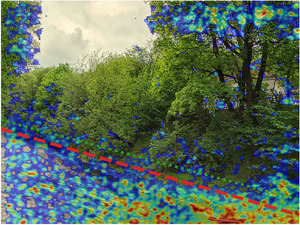
\includegraphics{sgbp/thumb/pano_addlmffiaizqlx-0.jpg}
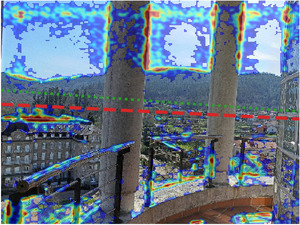
\includegraphics{sgbp/thumb/pano_addontedcyafqk-6.jpg}
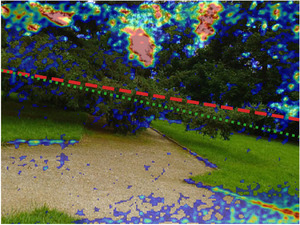
\includegraphics{sgbp/thumb/pano_addpqpwdfajota-4.jpg}
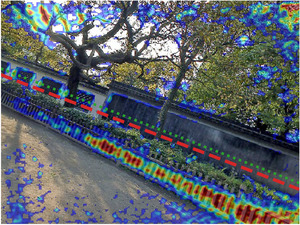
\includegraphics{sgbp/thumb/pano_addqflfuthjcbf-3.jpg}
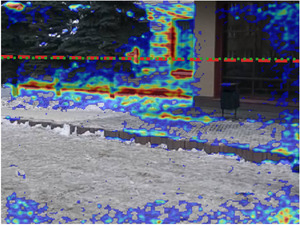
\includegraphics{sgbp/thumb/pano_addsqkgygrcixb-3.jpg}
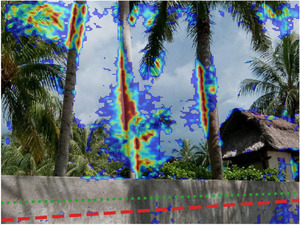
\includegraphics{sgbp/thumb/pano_addtdiecjavkue-1.jpg}
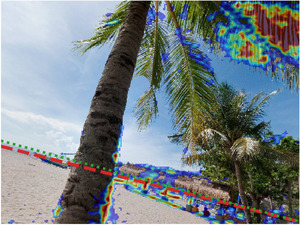
\includegraphics{sgbp/thumb/pano_addtdiecjavkue-3.jpg}
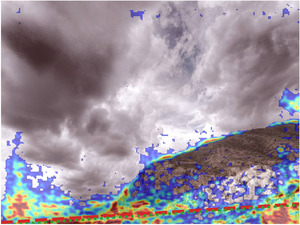
\includegraphics{sgbp/thumb/pano_addtfngrqwwyvb-6.jpg}
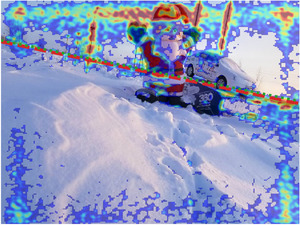
\includegraphics{sgbp/thumb/pano_addtwdtklktubg-3.jpg}
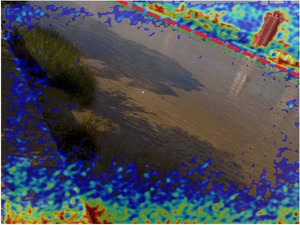
\includegraphics{sgbp/thumb/pano_adqwuqgahcnffm-0.jpg}
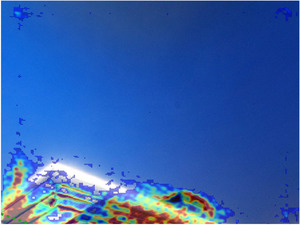
\includegraphics{sgbp/thumb/pano_ayflzrhzcccird-0.jpg}
\includegraphics{sgbp/thumb/pano_ayflzrhzcccird-1.jpg}
\includegraphics{sgbp/thumb/pano_ayflzrhzcccird-2.jpg}
\includegraphics{sgbp/thumb/pano_ayflzrhzcccird-3.jpg}
\includegraphics{sgbp/thumb/pano_ayflzrhzcccird-4.jpg}
\includegraphics{sgbp/thumb/pano_ayflzrhzcccird-5.jpg}
\includegraphics{sgbp/thumb/pano_ayflzrhzcccird-6.jpg}
\includegraphics{sgbp/thumb/pano_ayfnoupsclgjpp-3.jpg}
\includegraphics{sgbp/thumb/pano_ayfnoupsclgjpp-4.jpg}
\includegraphics{sgbp/thumb/pano_ayfnoupsclgjpp-5.jpg}
\includegraphics{sgbp/thumb/pano_ayfnoupsclgjpp-6.jpg}

\clearpage

\protect\hypertarget{study}{}{}

\hypertarget{user-study-examples}{%
\section{User Study Examples}\label{user-study-examples}}

In this section, we present additional pairs of images shown during the
user study along with their distorted parameter(s), extending the
results shown in fig.~\ref{fig:pstudy_overall_sensitivity}.

Note that in the study, the image containing the virtual object inserted using the
ground truth camera calibration was randomly positioned left or right.


\begin{minipage}{\linewidth}
\centering
\vspace{1em}
Ground truth calibration\hspace{0.2\linewidth}Distorted calibration\\\vspace{0.5em}
\includegraphics[width=0.45\linewidth]{study/thumb/pano_ahxngimugqzaln-1_4_gt.jpg}
\includegraphics[width=0.45\linewidth]{study/thumb/pano_ahxngimugqzaln-1_4_dc.jpg}\\
Distorted parameter(s): hfov\\
Amount: -30.76$^\circ$
\end{minipage}

\begin{minipage}{\linewidth}
\centering
\hrule\vspace{1em}
Ground truth calibration\hspace{0.2\linewidth}Distorted calibration\\\vspace{0.5em}
\includegraphics[width=0.45\linewidth]{study/thumb/pano_ahxngimugqzaln-1_5_gt.jpg}
\includegraphics[width=0.45\linewidth]{study/thumb/pano_ahxngimugqzaln-1_5_dc.jpg}\\
Distorted parameter(s): roll, hfov\\
Amount: -7.17$^\circ$, -44.48$^\circ$
\end{minipage}

\begin{minipage}{\linewidth}
\centering
\hrule\vspace{1em}
Ground truth calibration\hspace{0.2\linewidth}Distorted calibration\\\vspace{0.5em}
\includegraphics[width=0.45\linewidth]{study/thumb/pano_ahxngimugqzaln-1_6_gt.jpg}
\includegraphics[width=0.45\linewidth]{study/thumb/pano_ahxngimugqzaln-1_6_dc.jpg}\\
Distorted parameter(s): roll\\
Amount: 13.04$^\circ$
\end{minipage}

\begin{minipage}{\linewidth}
\centering
\hrule\vspace{1em}
Ground truth calibration\hspace{0.2\linewidth}Distorted calibration\\\vspace{0.5em}
\includegraphics[width=0.45\linewidth]{study/thumb/pano_ahxngimugqzaln-1_7_gt.jpg}
\includegraphics[width=0.45\linewidth]{study/thumb/pano_ahxngimugqzaln-1_7_dc.jpg}\\
Distorted parameter(s): pitch, roll\\
Amount: -16.58$^\circ$, -1.69$^\circ$
\end{minipage}

\begin{minipage}{\linewidth}
\centering
\hrule\vspace{1em}
Ground truth calibration\hspace{0.2\linewidth}Distorted calibration\\\vspace{0.5em}
\includegraphics[width=0.45\linewidth]{study/thumb/pano_ahxngxlbcrplaw-6_0_gt.jpg}
\includegraphics[width=0.45\linewidth]{study/thumb/pano_ahxngxlbcrplaw-6_0_dc.jpg}\\
Distorted parameter(s): roll, hfov\\
Amount: 14.04$^\circ$, 32.35$^\circ$
\end{minipage}

\begin{minipage}{\linewidth}
\centering
\hrule\vspace{1em}
Ground truth calibration\hspace{0.2\linewidth}Distorted calibration\
\includegraphics[width=0.45\linewidth]{study/thumb/pano_ahxngxlbcrplaw-6_1_gt.jpg}
\includegraphics[width=0.45\linewidth]{study/thumb/pano_ahxngxlbcrplaw-6_1_dc.jpg}\\
Distorted parameter(s): roll\\
Amount: 3.30$^\circ$
\end{minipage}

\begin{minipage}{\linewidth}
\centering
\hrule\vspace{1em}
Ground truth calibration\hspace{0.2\linewidth}Distorted calibration\\\vspace{0.5em}
\includegraphics[width=0.45\linewidth]{study/thumb/pano_ahxngxlbcrplaw-6_2_gt.jpg}
\includegraphics[width=0.45\linewidth]{study/thumb/pano_ahxngxlbcrplaw-6_2_dc.jpg}\\
Distorted parameter(s): pitch, roll, hfov\\
Amount: 24.13$^\circ$, 4.30$^\circ$, 12.24$^\circ$
\end{minipage}

\begin{minipage}{\linewidth}
\centering
\hrule\vspace{1em}
Ground truth calibration\hspace{0.2\linewidth}Distorted calibration\\\vspace{0.5em}
\includegraphics[width=0.45\linewidth]{study/thumb/pano_ahxngxlbcrplaw-6_3_gt.jpg}
\includegraphics[width=0.45\linewidth]{study/thumb/pano_ahxngxlbcrplaw-6_3_dc.jpg}\\
Distorted parameter(s): roll\\
Amount: -1.46$^\circ$
\end{minipage}

\begin{minipage}{\linewidth}
\centering
\hrule\vspace{1em}
Ground truth calibration\hspace{0.2\linewidth}Distorted calibration\\\vspace{0.5em}
\includegraphics[width=0.45\linewidth]{study/thumb/pano_ahxngxlbcrplaw-6_4_gt.jpg}
\includegraphics[width=0.45\linewidth]{study/thumb/pano_ahxngxlbcrplaw-6_4_dc.jpg}\\
Distorted parameter(s): roll\\
Amount: -4.49$^\circ$
\end{minipage}

\begin{minipage}{\linewidth}
\centering
\hrule\vspace{1em}
Ground truth calibration\hspace{0.2\linewidth}Distorted calibration\\\vspace{0.5em}
\includegraphics[width=0.45\linewidth]{study/thumb/pano_ahxnzyleoiflya-0_5_gt.jpg}
\includegraphics[width=0.45\linewidth]{study/thumb/pano_ahxnzyleoiflya-0_5_dc.jpg}\\
Distorted parameter(s): roll\\
Amount: 15.65$^\circ$
\end{minipage}

\begin{minipage}{\linewidth}
\centering
\hrule\vspace{1em}
Ground truth calibration\hspace{0.2\linewidth}Distorted calibration\\\vspace{0.5em}
\includegraphics[width=0.45\linewidth]{study/thumb/pano_ahxnzyleoiflya-0_6_gt.jpg}
\includegraphics[width=0.45\linewidth]{study/thumb/pano_ahxnzyleoiflya-0_6_dc.jpg}\\
Distorted parameter(s): hfov\\
Amount: 21.62$^\circ$
\end{minipage}


\clearpage

\FloatBarrier

\protect\hypertarget{studyresults}{}{}

\hypertarget{user-study-results}{%
\section{User Study Results}\label{user-study-results}}

In this section, we present additional results from the user study,
extending the results shown in fig.~\ref{fig:pstudy_overall_sensitivity}. Specifically, we show the human
sensitivity with respect to errors and values of each parameter against
one another.

\begin{figure}[!ht]
\centering
\includegraphics[width=\linewidth]{study_results/hist2d_image_units_error_error.png}\\
\caption[Influence of parameter errors on human sensitivity]{Influence of parameter errors between themselves on human
sensitivity to errors. We bin the percentage of people choosing the
ground truth per image of the user study. The colors in the plot
represents the median over all values in each bin. 100\% (yellow) means
humans always detect the distortion, 50\% (blue) means total confusion,
where humans statistically selects the distorted image as often as the
ground truth.}
\end{figure}

\begin{figure}[!ht]
\centering
\includegraphics[width=\linewidth]{study_results/hist2d_image_units_error_value.png}\\
\caption[Influence of parameter errors wrt. other parameter values on human sensitivity]{Influence of parameter errors wrt. other parameter values on
human sensitivity to errors.}
\end{figure}

\begin{figure}[!ht]
\centering
\includegraphics[width=\linewidth]{study_results/hist2d_image_units_value_error.png}\\
\caption[Influence of parameter values wrt. other parameter errors on
human sensitivity]{Influence of parameter values wrt. other parameter errors on
human sensitivity to errors.}
\end{figure}

\begin{figure}[!ht]
\centering
\includegraphics[width=\linewidth]{study_results/hist2d_image_units_value_value.png}\\
\caption[Influence of parameter values between themselves on human sensitivity]{Influence of parameter values between themselves on human
sensitivity to errors. Note how when the roll parameter has a value very
close to 0$^\circ$, humans could detect distortions more easily, whereas larger
roll value (image tilted around the viewing axis) yields lower detection
rate by humans.}
\end{figure}

\FloatBarrier

\protect\hypertarget{voi}{}{}

\hypertarget{virtual-object-insertions}{%
\section{Virtual object insertions}\label{virtual-object-insertions}}

In this section, we present additional virtual object insertions,
extending the results shown in fig.~\ref{fig:applications_virtual_object_insertion}.


\begin{multicols}{3}
\includegraphics[width=\linewidth]{virtual_object_insertions/pano_abpaafvavryivl-2_0_es.jpg}\vspace{1em}
\includegraphics[width=\linewidth]{virtual_object_insertions/pano_abpaafvavryivl-2_1_es.jpg}\vspace{1em}
\includegraphics[width=\linewidth]{virtual_object_insertions/pano_abpaafvavryivl-2_6_es.jpg}\vspace{1em}
\includegraphics[width=\linewidth]{virtual_object_insertions/pano_abpebgbgmpccye-6_0_es.jpg}\vspace{1em}
\includegraphics[width=\linewidth]{virtual_object_insertions/pano_abpebgbgmpccye-6_1_es.jpg}\vspace{1em}
\includegraphics[width=\linewidth]{virtual_object_insertions/pano_abpebgbgmpccye-6_4_es.jpg}\vspace{1em}
\includegraphics[width=\linewidth]{virtual_object_insertions/pano_abpebgbgmpccye-6_6_es.jpg}\vspace{1em}
\includegraphics[width=\linewidth]{virtual_object_insertions/pano_abpezaevuxprln-0_5_es.jpg}\vspace{1em}
\includegraphics[width=\linewidth]{virtual_object_insertions/pano_abpezaevuxprln-0_7_es.jpg}\vspace{1em}
\includegraphics[width=\linewidth]{virtual_object_insertions/scene0_compose.jpg}\vspace{1em}
\includegraphics[width=\linewidth]{virtual_object_insertions/scene107_compose.jpg}\vspace{1em}
\includegraphics[width=\linewidth]{virtual_object_insertions/scene123_compose.jpg}\vspace{1em}
\includegraphics[width=\linewidth]{virtual_object_insertions/scene156_compose2.jpg}\vspace{1em}
\includegraphics[width=\linewidth]{virtual_object_insertions/scene27_compose.jpg}\vspace{1em}
\end{multicols}


\protect\hypertarget{ablative}{}{}

\hypertarget{ablative-study}{%
\section{Ablative study}\label{ablative-study}}

In this section, we compare the performance obtained by our method when all parameters are trained jointly versus separately. We observe that joint training leads to an improvement over every parameter over most ranges.


\begin{figure}[!ht]
\centering
\includegraphics[width=\linewidth]{ablative/ablative.png}
\caption{Comparison between joint and separate parameters optimization.}
\end{figure}
